\chapter{Dynamical Three-Field Model}
\label{ch:dynamical_threefield}

\begin{flushright}
Think you're escaping and run into yourself. \\Longest way round is the shortest way home. \\
James Joyce, \emph{Ulysses}
\end{flushright}

\section{Review and Motivation}
\label{secReview}

We assume that four-dimensional QCD can be modeled by the following five-dimensional action, written in the string frame:
\ba
\cS &=&\frac{1}{16\pi G_5} \int d^5x \sqrt{-g} e^{-2\Phi}  \Bigg( R+4\partial_M\Phi\partial^M\Phi \nonumber \\ 
& & \mbox{} - \mathrm{Tr} \left[ |DX|^2  +\partial_M \mathcal{G} \partial^M \mathcal{G} + \frac{1}{2g_5^2} (F_A^2+F_V^2) +V_m(\Phi,X^2, \mathcal{G}) \right]\Bigg) \, .
\label{eqStringAction}
\ea
Here $\Phi$ is the dilaton and the metric is pure AdS, $g_{MN}=z^{-2}\eta_{MN},$ with the AdS curvature defined to be unity.
The constant $g_5^2 = 12\pi^2/N_c$, where $N_c$ is the number of colors.
The covariant derivative is defined as $D_M = \partial_M+i[V_M,X]-i\{A_M,X\}$.
The scalar field $X$, which is dual to the $\bar{q}q$ operator, obtains a $z$-dependent vacuum expectation value (VEV)
\be
\langle X \rangle=\frac{\chi(z)}{2}I \, ,
\ee
where $I$ is the $2 \times 2$ identity matrix.
The glueball field $\mathcal{G}$ similarly obtains a $z$-dependent VEV, $G(z)$.
We examine the background dynamics of the fields
\be
\cS =\frac{1}{16\pi G_5} \int d^5x \sqrt{-g} e^{-2\Phi}  \left(R+4\partial_M\Phi\partial^M\Phi -\thalf\partial_M \chi \partial^M \chi -\thalf\partial_M G \partial^M G -V(\Phi,\chi,G) \right) \, ,
\ee
where $V=\mathrm{Tr}[V_m]$.
The scalar fields $\Phi,\chi,G$ are dimensionless. 

It is easier to search for the background fields in the Einstein frame, where the vacuum action takes the canonical form
\be
\cS_E=\frac{1}{16\pi G_5} \int d^5x \sqrt{-\tilde{g}}\left(\tilde{R}-\thalf\partial_M\phi\partial^M\phi -\thalf\partial_M\chi\partial^M\chi -\thalf\partial_M G \partial^M G - \tilde{V}(\phi,\chi,G)\right) \, .
\label{eq:Einstein}
\ee
The tilde distinguishes the two frames, with $\tilde{V}=e^{4\Phi/3}V,$ and the dilaton is rescaled for a canonical action $\phi=\sqrt{8/3}\Phi$.
The string and Einstein frame metrics are related by the conformal transformation
\be
g_{MN}=e^{2\phi/\sqrt{6}}\tilde{g}_{MN} \, .
\ee

Previous work showed how to construct a potential for a gravity-dilaton-chiral system without the glueball condensate. 
We examine the behavior assuming that the fields have power-law behavior, which is accurate in both the UV and IR limits \cite{Springer2010}. 
One of the equations of motion is independent of the choice of potential,
\be
\chidot^2  = \frac{\rt6}{z^2} \Dz(z^2\phidot) \, . 
\label{twofield}
\ee
To obtain linear confinement, the dilaton should have quadratic behavior in the IR limit, $\phi(z)=\lambda z^2$.
The chiral field should have linear behavior in the IR, $\chi(z)=A z$, where $A$ sets the mass splitting between the axial-vector and vector mesons for large radial quantum numbers $n$. 
This constant mass-splitting at large $n$ occurs because of the non-restoration of chiral symmetry \cite{Shifman-2008}.
Inserting this into (\ref{twofield}), we find that the chiral field behaves as
\be
\chi(z)=6^{3/4}\sqrt{\lambda}z \, ,
\ee
which removes one of the independent parameters of the model in \cite{gherghetta-kelley}. 
Using the phenomenological value of $\lambda$, which determines the slope of the radial Regge trajectories, we find a mass splitting that is much too large.
Because this problem arises in the equation that is independent of the potential, this issue cannot be resolved by the choice of potential in models that do not consider the glueball condensate. 
Models that derive the field behavior using the superpotential method suffer from the same problem.

To resolve this problem, we consider the effects of the glueball condensate $G$ on the background equations. 
This field must be linear in the IR for linear confinement, and behave as $G \sim z^4$ in the UV to match the operator dimension in the AdS/CFT dictionary.

It is noted that the model proposed by Huang and Li \cite{Li2013, Li2013a} accurately represents the non-restoration of chiral symmetry using a model with only two background fields, but their model differs from the work presented here in several respects.
They place the meson fields and chiral dynamics in the open-string sector of the model. 
For linear confinement, this requires that the chiral field approach a constant in the IR, which necessitates a modified metric to obtain the correct chiral dynamics.
Our model allows the metric to remain purely AdS in the string frame.
Finally, they do not determine an explicit form of the potential, which is the central goal of this work.

%%%%%%%%%%%%%%%%%%%%%
\section{Construction of Potential}
\label{sec:potential}

Consider the action in the Einstein frame (\ref{eq:Einstein}).
To simplify the equations of motion, we use a transformed potential, 
\be
V=e^{-2\phi/\rt6}\tilde{V} \, .
\label{transform}
\ee
This is simply the potential in the string frame.
We re-write it as
\be
V = -12 + 4\sqrt{6}\phi + a_0\phi^2 +\frac{m_X^2}{2}\chi^2 + U \,.
\label{V}
\ee
Here $U$ is more than quadratic in the fields. 
 The AdS/CFT dictionary sets the mass for the fields according to the dimension of the dual operator,
\be
m^2L^2=\Delta(\Delta-4) \,,
\ee
where $L$ is the AdS curvature which we set to unity.  The dimension of the $q\bar{q}$ operator is 3, so $m_X^2 = -3/L^2$.
The dilaton mass is undetermined and is not connected to the dimension of the corresponding operator, as discussed in \cite{Springer2010}.  
It is related to the parameter $a_0$ by $a_0 = \thalf \left[ \mL2-8 \right]$. 
The potential should be an even function of $\chi$. 

The equations of motion can be written as
\be
\chidot^2 + \Gdot^2 = \frac{\rt6}{z^2} \Dz(z^2\phidot) \, ,
\label{C}
\ee
\be
U=\thalf \rt6 z^2 \phiddot - \tthalf (z\phidot)^2 - 3 \rt6 z\phidot 
-4\sqrt{6}\phi - a_0\phi^2 +\tthalf\chi^2 \, ,
\label{U}
\ee
\be
 \frac{\partial U}{\partial \phi}=3z\phidot - 2a_0\phi \, ,
\label{phi}
\ee
\be
 \frac{\partial U}{\partial \chi}
=z^2\chiddot -3z\chidot \left(1+\frac{z\phidot}{\rt6} \right) + 3\chi \, ,
\label{chi}
\ee
\be
 \frac{\partial U}{\partial G}=
z^2\Gddot -3z\Gdot \left(1+\frac{z\phidot}{\rt6} \right) \, .
\label{G}
\ee
We assume that the potential has no explicit dependence on the coordinate $z$,  so the equations \ref{phi}-\ref{G} are not independent, and we can eliminate one. 

%%%%%%%%%%%%%%%%%%%%%
\subsection{Infrared Limit}

The requirement of linear confinement requires a solution in the large $z$ limit of the  form
\ba
\phi &=& \lambda z^2 \, , \\
\chi &=& Az \, , \\
G &=& B z \, .
\label{Lz}
\ea
Substitution into (\ref{C}) gives
\be
A^2 + B^2 = 6\rt6 \lambda \, .
\label{Clarge}
\ee
The parameter $\lambda$ is fixed by the slope of the linear trajectory and $A$ is fixed by the axial-vector -- vector mass difference.  
It is useful to write these as
\bd
A = 6^{3/4} \sqrt{\lambda} \cos\theta \, ,
\ed
\be
B = 6^{3/4} \sqrt{\lambda} \sin\theta \, ,
\ee
where $\theta$ now becomes the parameter controlling the axial-vector -- vector mass splitting.
Inserting (\ref{Lz}) into (\ref{U}-\ref{G}) suggests the following terms in our ansatz for the potential
\be
U =  a_1 \phi \chi^2 + a_2 \phi G^2 + a_3 \chi^4 + a_4 G^4 + a_5 \chi^2 G^2 
+ a_6 G^2 \tanh(g\phi) \, .
\ee
We see that there must be a $G^2$ term in the IR limit, but this is forbidden in the weak-field limit because the glueball condensate field is massless. 
To circumvent this, we propose the term $G^2 \tanh(g\phi)$ with $g>0$.  
In the weak field limit this goes to $g\phi G^2$, which is acceptable.  
The $\tanh$ is suggested by \ref{transform}, and it provides a rapid exponential transition from the weak field to the strong field limits that is supported by phenomenology.
By substitution one finds the following constraints on the parameters:
\bd
U \rightarrow 6 + a_0 + 6\rt6 \left( \cos^2 \theta \, a_1 + \sin^2 \theta \, a_2 \right)
\ed
\be
+ 6^3 \left( \cos^4 \theta \, a_3 + \sin^4 \theta \, a_4 + \cos^2 \theta \sin^2 \theta \, a_5 \right) = 0 \, ,
\ee
\be
\frac{\partial U}{\partial \chi} \rightarrow
2a_1 + 24\rt6 \cos^2\theta \, a_3 + 12\rt6 \sin^2\theta \, a_5 + \rt6 = 0 \, ,
\ee
\be
\frac{\partial U}{\partial G} \rightarrow
2a_2 + 24\rt6 \sin^2\theta \, a_4 + 12\rt6 \cos^2\theta \, a_5 + \rt6 = 0 \, ,
\ee
\be
\frac{\partial U}{\partial G} \rightarrow a_6 = - \tthalf \, .
\label{LargeZ2}
\ee
We have chosen to exclude (\ref{phi}) because it is not independent. 
The parameter $a_6$ is determined, and the others will be determined by an examination of the UV limit.

%%%%%%%%%%%%%%%%%%%%%
\subsection{Ultraviolet Limit}

Next we look for a solution in the small $z$ limit. 
The AdS/CFT dictionary dictates that the leading-order UV behavior of the chiral and glueball condensate fields is determined by their dimension. 
Note also that we are working in the chiral limit where the quark mass is zero. 
We start by examining only the leading-order terms
\ba
\chi &=& \Sigma_0 z^3 \, ,\\
G &=& G_0 z^4 \, .
\ea
Substitution into (\ref{C}) and imposing the boundary condition $\phi(0)=0$ gives
\be
\phi = \frac{\rt6}{28} \Sigma_0^2 z^6 + \frac{\rt6}{27} G_0^2 z^8 \, .
\label{Sz}
\ee

Substitution of the desired solution into eqs. (\ref{U})-(\ref{G}) results in
\be
\tilde{U} = -\tthalf (z\phidot)^2 - a_0\phi^2
\ee
\be
\frac{\partial \tilde{U}}{\partial \phi} = \frac{\rt6}{14} (9-a_0) \Sigma_0^2 z^6 + \frac{2\rt6}{27} (12-a_0) G_0^2 z^8
\ee
\be
\frac{\partial \tilde{U}}{\partial \chi} = -9\Sigma_0 \left( \frac{3}{14} \Sigma_0^2 + \frac{8}{27} G_0^2 z^2 \right) z^9
\ee
\be
\frac{\partial \tilde{U}}{\partial G} = -12G_0 \left( \frac{3}{14} \Sigma_0^2 + \frac{8}{27} G_0^2 z^2 \right) z^{10}
\ee
By substitution one finds the following constraints on the parameters:
\ba
\frac{\partial \tilde{U}}{\partial \phi} &\rightarrow& 3a_0 + 7\rt6 a_1 - 27 = 0 \label{dUdphi1} \\
&{\rm and}& 4a_0 + 9\rt6 (a_2 + g a_6) - 48 = 0 \label{dUdphi2}
\ea
\ba
\frac{\partial \tilde{U}}{\partial \chi} &\rightarrow& \rt6 a_1 + 56 a_3 + 27 = 0 \\
&{\rm and}& \rt6 a_1 + 27 a_5 + 36 = 0
\ea
\ba
\frac{\partial \tilde{U}}{\partial G} &\rightarrow& \rt6 (a_2 + g a_6) + 28 a_5 + 36 = 0 \label{dUdG1}\\
&{\rm and}& \rt6 (a_2 + g a_6) + 54 a_4 + 48 = 0 \label{dUdG2}
\ea

Using only this leading-order behavior in (\ref{U}-\ref{G}), the system of equations is inconsistent, as there are more equations from matching powers of $z$ than unknown parameters. 
There are three equations from the IR limit and 6 equations from the UV limit, for a total of nine equations to be solved by only 8 parameters, $a_0 - a_5$, $a_8$ and $g$.  
To solve this problem, consider adding a term $\Sigma_n z^n$ to $\chi$.  
Substituting into (\ref{C}) and keeping only the lowest-order cross-term we find the additional term in $\phi$
\be
\Delta \phi = \frac{\rt6 n \Sigma_0 \Sigma_n}{(n+4)(n+3)} z^{n+3} \, .
\ee
From (\ref{U}) we find that
\be
U = -\tthalf (z\phidot)^2 - a_0\phi^2 +3 \frac{n^3 -13n +12}{(n+4)(n+3)} \Sigma_0 \Sigma_n z^{n+3} \, .
\ee
Since the $\phi^2$ terms start out as $z^{12}$, $z^{14}$, $z^{16}$, and so do the terms in the potential, the $n$ can only take the values 9, 11, etc.  
This term contributes only to the equation for $\partial U/\partial \chi$.
\be
\frac{\partial U}{\partial \chi} = -9\Sigma_0 \left( \frac{3}{14} \Sigma_0^2 + \frac{8}{27} G_0^2 z^2 \right) z^9 + (n-3)(n-1) \Sigma_n z^n \, .
\ee
By power counting both $n=9$ and $n=11$ can contribute.  

There could also be higher order terms in $G$ such as $G_m z^m$.  
This leads to the additional term in $\phi$
\be
\Delta \phi = \frac{8 m G_0 G_m}{\rt6 (m+5)(m+4)} z^{m+4} \, .
\ee
It contributes to the equation for $\partial U/\partial G$ as
\be
\frac{\partial U}{\partial G} = -12G_0 \left( \frac{3}{14} \Sigma_0^2 + \frac{8}{27} G_0^2 z^2 \right) z^{10}
+ m (m-4) G_n z^m \, .
\ee
The choice $m=8$ is not possible as there is no term of the same order to balance it.  
Terms with $m=10$ and $m=12$ are possible.  
These new terms cannot affect the equation for $\partial U/\partial \phi$  nor can they contribute to the equation for $\partial U/\partial \chi$.  
Considering higher order terms in both $\chi$ and $G$ leads to
\be
U = -\tthalf (z\phidot)^2 - a_0\phi^2 +3 \frac{n^3 -13n +12}{(n+4)(n+3)} \Sigma_0 \Sigma_n z^{n+3}
+ \frac{4m(m-4)}{m+4} G_0 G_m z^{m+4} \, .
\ee 
The appearance of these terms can be understood by writing the following schematic expansions.
\bd
\chi \sim \Sigma_0 z^3 + \Sigma_0^3 z^9 + G_0^2 \Sigma_0 z^{11} + \cdot\cdot\cdot
\ed
\bd
G \sim G_0 z^4 + \Sigma_0^2 G_0 z^{10} + G_0^3 z^{12} + \cdot\cdot\cdot
\ed
That is, $\chi$ is an odd function of $\Sigma_0$ and $G$ is an odd function of $G_0$.  
These are the symmetries in the equations of motion.  
They also follow the spirit of the AdS/CFT correspondence in terms of the dimensionality of the operators and the powers of $z$.

Including now $m$ = 10 and 12, and $n$ = 9 and 11, we have the following set of equations in the small $z$ limit, where LHS and RHS refer to the left and right sides of the respective equations:
\ba
U_{\rm LHS} &=& 3 \Sigma_0^4 z^{12} \left[ 4 \frac{\Sigma_9}{\Sigma_0^3} - \frac{(54+a_0)}{2^3 \cdot 7^2} \right] \nonumber \\
&+& \frac{1}{7} \Sigma_0^2 G_0^2 z^{14} \left[ 120 \frac{G_{10}}{\Sigma_0^2 G_0} + 120 \frac{\Sigma_{11}}{\Sigma_0 G_0^2} - \frac{(72+a_0)}{9} \right] \nonumber \\
&+& 2G_0^4 z^{16} \left[ 12 \frac{G_{12}}{G_0^3} - \frac{(96+a_0)}{3^5} \right] \, ,
\ea
\ba
U_{\rm RHS} &=& \Sigma_0^4 z^{12} \left[  \frac{\rt6}{28} a_1 + a_3\right] \nonumber \\
&+& \Sigma_0^2 G_0^2 z^{14} \left[ \frac{\rt6}{27} a_1 + \frac{\rt6}{28} (a_2 + g a_6) + a_5 \right] \nonumber \\
&+& G_0^4 z^{16} \left[ \frac{\rt6}{27} (a_2 + g a_6) + a_4 \right] \, .
\ea
\ba
\left(\frac{\partial U}{\partial \chi}\right)_{\rm LHS} &=& 3 \Sigma_0^3 z^9 \left[ -\frac{9}{14} + 16 \frac{\Sigma_9}{\Sigma_0^3} \right]+ 8 \Sigma_0 G_0^2 z^{11} \left[ - \frac{1}{3} + 10 \frac{\Sigma_{11}}{\Sigma_0 G_0^2} \right] \, , \\
\left(\frac{\partial U}{\partial \chi}\right)_{\rm RHS} &=& \Sigma_0^3 z^9 \left[ \frac{\rt6}{14} a_1 + 4 a_3  \right]+ \Sigma_0 G_0^2 z^{11} \left[  \frac{2\rt6}{27} a_1 + 2 a_5 \right] \, .
\ea
\ba
\left(\frac{\partial U}{\partial G}\right)_{\rm LHS} &=& 6 \Sigma_0^2 G_0 z^{10} \left[ -\frac{3}{7} + 10 \frac{G_{10}}{\Sigma_0^2 G_0} \right]
+ 32 G_0^3 z^{12} \left[ - \frac{1}{9} + 3 \frac{G_{12}}{G_0^3} \right] \, , \\
\left(\frac{\partial U}{\partial G}\right)_{\rm RHS} &=& \Sigma_0^2 G_0 z^{10} \left[ \frac{\rt6}{14} (a_2 + g a_6) + 2a_5 \right] \\
&+& G_0^3 z^{12} \left[ \frac{2\rt6}{27}  (a_2 + g a_6) + 4a_4 \right] \, .
\ea

Altogether, from both the UV and IR limits, there are ten independent equations for the twelve parameters $a_0 - a_6$, $\Sigma_9$, $\Sigma_{11}$, $G_{10}$, $G_{12}$, and $g$.  
We take $g$ as the free parameter to use as the rate of transition from small $z$ to large $z$.  
The parameters in the potential are found to be
\ba
a_0 &=&  \frac{3}{2} \frac{1}{6 + \sin^2 \theta}\left[ 120 + 62 \sin^2 \theta + 63 \rt6 g \sin^2 \theta \right] \, , \\
a_1 &=&  -\frac{3\rt6}{4} \frac{1}{6 + \sin^2 \theta}\left[ 12 + 8 \sin^2 \theta + 9 \rt6 g \sin^2 \theta \right] \, , \\
a_2 &=&  -\frac{\rt6}{4} \frac{1}{6 + \sin^2 \theta}\left[ 32 + 24 \sin^2 \theta + 3 \rt6 g(9 \sin^2 \theta - 2) \right] \, ,
\ea
\be
2 a_3 \cos^2 \theta + a_5 \sin^2 \theta = \frac{1}{24} \frac{1}{6 + \sin^2 \theta}\left[ 24 + 22 \sin^2 \theta + 27 \rt6 g \sin^2 \theta \right] \, ,
\ee
\be
2 a_4 \sin^2 \theta + a_5 \cos^2 \theta = \frac{1}{24} \frac{1}{6 + \sin^2 \theta}\left[ 20 +22 \sin^2 \theta   +  3 \rt6 g (9 \sin^2 \theta -2) \right] \, ,
\ee
\be
a_6 = -\frac{3}{2} \, .
\ee
The coefficients $a_0$, $a_1$, $a_2$ and $a_6$ are determined, while there are two equations for the three coefficients $a_3$, $a_4$ and $a_5$.  
That leaves $a_5$ as a free parameter, to be fit numerically, along with $g$, $\theta$, $G_0$, $\Sigma$, and $\lambda$.

%%%%%%%%%%%%%%%%%%%%%
\section{Numerical Solution}
\label{sec:numerical_solution}

Using the potential discussed, we seek a numerical solution that simultaneously satisfies the UV and IR limits. 
We use equations (\ref{C}, \ref{chi}, \ref{G}), which allows for an additional term in the potential, $\Delta U$, such that 
\be
\frac{\partial }{\partial \chi} \Delta U = \frac{\partial }{\partial G}\Delta U = 0 \, ,
\ee
which will be determined from the numerical solution.

The differential equations represent a stiff system, and treatment of the problem as an initial value problem leads to numerical instabilities. 
We treat it instead as a boundary value problem, using Dirichlet boundary conditions at both boundaries. 
A relaxation method is used in combination with input approximations for the background fields, which are then iterated to find a stable solution to the system with the given boundary conditions. 
Because the system is nonlinear, the solution found is not guaranteed to be unique.

The IR boundary is chosen to be sufficiently large to capture the infrared behavior and to give accurate Regge behavior for the large-$n$ radial excitations of the mesons. 
The UV boundary should approach zero, but it cannot reach zero because of the singularity in the equations of motion. 
This becomes a problem because equation (\ref{C}) allows constant and divergent terms 
\be
\Delta \phi(z) = c_1 + c_2 z^{-1} \, .
\ee
Symbolically, these terms can be set to zero by enforcing the Dirichlet boundary condition $\phi(0)=0$, but this is impossible to enforce numerically. 
Creative choice of UV boundary conditions can eliminate one, but not both, of these unwanted terms without affecting the chiral and glueball fields. 
The behavior of the numerical solutions suggests that the desired UV behavior is an unstable solution to the equations, and therefore difficult or impossible to find with this iterative method.

As an alternative to direct solution, we parameterize the fields as follows:
\be
\Psi(z) = \psi(z)_{UV} f(z) + \psi(z)_{IR} \left(1-f(z)\right) \, .
\ee
Here $f(z)$ is some function that transitions smoothly from 1 at small values of $z$ to 0 at large $z$, while $\psi(z)_{xy}$ represents the known UV and IR limits of the fields $\phi, \chi,$ and $G$. 
The switching functions need not be the same for each field. We choose 
\ba
f_\phi(z)&=&e^{-(\beta_1z)^{10}} \, , \\ \label{param1}
f_\chi(z)&=&e^{-(\beta_2z)^4} \, , \\  \label{param2}
f_G(z)&=&e^{-(\beta_3z)^5} \, . \label{param3}
\ea
The powers of the exponential are chosen to be greater than the known power-law behavior of the fields in the UV limit so as to not interfere with this behavior. 
The $\beta_i$ will be determined by numerical fitting.

The chiral condensate $\Sigma$ is set using the Gell-Mann--Oakes--Renner relation:
\be
(m_u+m_d)\Sigma = f_\pi^2 m_\pi^2 \, .
\ee
Using $m_\pi = 139.6$ MeV, $f_\pi = 92 $ MeV, and $m_u+m_d = 7.0 $ MeV yields a value of $\Sigma = (286\, \mathrm{MeV})^3$.

In all, we have eight parameters to be determined numerically. 
The first constraint is to obtain the best global visual fit to the vector and axial-vector meson spectra.   
We do not simply do a chi-squared fitting to the experimental data because the measurement error for the ground state $\rho$ meson is so much smaller than for the others that this would effectively act as the only constraint. 
Second, we seek to minimize the error in the finite-difference approximations to equations $\ref{C}, \ref{chi},$ and $\ref{G}$.  
This is done to an accuracy of one part in $10^4$. 

Three of the parameters are most phenomenologically relevant: $\lambda,$ which controls the slope of the meson spectra in the large-$n$ limit; $\theta,$ which controls the mass splitting between the $a_1$ and $\rho$ mesons at large $n$, and $\beta_2$, which controls the location of the ``bend" in the $a_1$ spectrum.
For each set of these parameters, the other parameters are determined by a routine that minimizes the error in the equations of motion. 
The parameters found are shown in Table \ref{tabParam}.

\begin{table}[htb]
\begin{center}
\begin{tabular}{| l | c || c | c | }
\hline
  $\lambda^{1/2}$ & $304$ MeV & $\beta_1$ & 3.04 GeV  \\
  $G_0^{1/4}$ & 552 MeV & $\beta_2$ & 274 MeV \\
  $ \theta $& 1.44 & $\beta_3$ & 558 MeV \\
  $g $& 3.20 & $a_5$ & 1.63 \\
  \hline
\end{tabular}
\caption{Best fit parameters for the phenomenological model. 
The parameters $\lambda, \theta,$ and $ \beta_2$ are chosen for the best visual fit to the $\rho$ and $a_1$ data, with the rest set by minimizing the error in the equations of motion (\ref{C}), (\ref{chi}-\ref{G}). }
\label{tabParam}
\end{center}
\end{table}

The background fields that are obtained from this analysis are shown in Figures \ref{figDilaton}-\ref{figGlueball}. 
The asymptotic power-law behavior of the fields is evident in the linear portions of the log-log scale plots shown.
 The ``transition" behavior is most evident in the dilaton because of the large value of $\beta_1$, which controls the value of $z$ at which the field transitions from the UV limit to the IR limit. 

\clearpage

\begin{figure}[ht]
\center{\includegraphics[width=290pt]{dilaton.eps}}
\caption{A plot of the dilaton field $\Phi$ generated by the parameterization (\ref{param1}).
The UV and IR asymptotic behavior is apparent.
The coordinate $x$ is a dimensionless re-scaling of the conformal coordinate, $x=\sqrt{\lambda}z$.}
\label{figDilaton}
\end{figure}
\nopagebreak
\begin{figure}[*hb]
\center{\includegraphics[width=290pt]{chiral.eps}}
\caption{A plot of the chiral field $\chi$ generated by the parameterization (\ref{param2}). 
The UV and IR asymptotic behavior is apparent, with a rapid transition between them.
The coordinate $x$ is a dimensionless re-scaling of the conformal coordinate, $x=\sqrt{\lambda}z$.}
\label{figChiral}
\end{figure}

\clearpage

\begin{figure}[ht]
\center{\includegraphics[width=290pt]{glueball.eps}}
\caption{A plot of the glueball field $G$ generated by the parameterization (\ref{param3}).
The UV and IR asymptotic behavior is apparent, with a rapid transition between them.
The coordinate $x$ is a dimensionless re-scaling of the conformal coordinate, $x=\sqrt{\lambda}z$.}
\label{figGlueball}
\end{figure}
\nopagebreak
\begin{figure}[hb]
\center{\includegraphics[width=285pt]{deltaU.eps}}
\caption{Plot of the ``extra" term in the potential, $\Delta U(\phi)$. The solid line represents the numerical result, while the dashed line is the fitting of (\ref{eqFit}) using the parameters of Table \ref{deltaUfit}.}
\label{figdeltaU}
\end{figure}

\clearpage

We now analyze the ``extra" term in the potential, $\Delta U$. 
We obtain this term numerically by subtracting the right-hand side of \ref{U} from its left-hand side.
This term can be approximated numerically as a function of the dilaton field, 
\be
\Delta U\left(\phi\right) = \alpha_1 \phi^2 e^{-\left(\phi-\gamma_1\right)^2/\delta_1 } +   \alpha_2 \phi^2 e^{-\left(\phi-\gamma_2\right)^2/\delta_2 } \, .
\label{eqFit}
\ee
The best-fit values for these parameters are shown in Table \ref{deltaUfit}.  The $\Delta U$ as a function of $\phi$ is shown in Figure \ref{figdeltaU}.
\begin{table}[htb]
\begin{center}
\begin{tabular}{| l | r || l | r | }
\hline
$\alpha_1$ & $-3.043 \times 10^1$ & $\alpha_2$ & 2.671 $ \times 10^{-4}$ \\
$\gamma_1$ & 7.086 $\times 10^{-5}$ & $\gamma_2$ & 2.213 $ \times 10^{-2}$ \\ 
$\delta_1$ & 9.699 $ \times 10^{-5}$& $\delta_2$ & 1.471 $ \times 10^{-2} $\\ 
%$\alpha_2$ & 2.671 $ \times 10^{-4}$  \\
%$\gamma_2$ & 2.213 $ \times 10^{-2}$ \\
%$\delta_2$ & 1.471 $ \times 10^{-2} $\\
  \hline
\end{tabular}
\caption{The dimensionless parameters for the fitting to $\Delta U$.}
\label{deltaUfit}
\end{center}
\end{table}

\section{Summary}
In this chapter we discussed the construction of a potential for the background fields of a soft-wall AdS/QCD model. 
The shortcomings of a dynamical AdS/QCD model containing only the dilaton and chiral condensate fields, are alleviated by adding a glueball condensate to the model.
We analytically constructed a general potential $U(\phi,\chi,G)$ that recovers the necessary asymptotic behavior of the background fields.
Using this as a basis, we numerically constructed a potential that solves the selected background equations to within an accuracy of $10^{-4}$. 
There is an additional allowed term in the  potential, $\Delta U(\phi)$, that does not affect the equations that were used in the numerical procedure. 
This term was found numerically, and fit as a function of the dilaton field.

The potential as constructed here is not guaranteed to be unique.
If a different set of the background equations were chosen, the extra term would be expressed as a function of fields other than the dilaton.
The parameterization in (\ref{param1}-\ref{param3}) could also be chosen differently, resulting in a different potential but making little difference to the resulting meson spectra.
Finally, terms can be added that do not affect the equations of motion at all, namely, terms which satisfy 
\be
\Delta U = \Delta \frac{\partial U}{\partial \phi} = \Delta \frac{\partial U}{\partial \chi} = \Delta \frac{\partial U}{\partial G} =0 \, .
\ee

The background fields from this potential can be used to calculate mass spectra for the various light mesons.
This work will be presented in the next chapter.


